\documentclass[12pt,a4paper]{article}
\usepackage[legalpaper, portrait, margin=3cm]{geometry}
\usepackage{fancyhdr}
\usepackage{amsmath}
\usepackage{amssymb}
\usepackage{graphicx}
\usepackage{wrapfig}
\usepackage{blindtext}
\usepackage{hyperref}
\usepackage{biblatex}

\graphicspath{ {./} }
\hypersetup{
  colorlinks=true,
  linkcolor=blue,
  filecolor=magenta,
  urlcolor=blue,
  citecolor=blue,
  pdftitle={Relatório ASA - Projeto 1 - 2021/2022},
  pdfpagemode=FullScreen,
}
\addbibresource{./bibliography.bib}

\pagestyle{fancy}
\fancyhf{}
\rhead{Grupo \textbf{al007}}
\lhead{Relatório Projeto 1 ASA 2021/2022 LEIC-A}
\cfoot{Diogo Correia (99211) e Tomás Esteves (99341)}

\renewcommand{\footrulewidth}{0.2pt}

\renewcommand{\labelitemii}{$\circ$}
\renewcommand{\labelitemiii}{$\diamond$}

\begin{document}
  \section{Descrição do Problema e da Solução}

  Para o \textbf{problema 1} utilizou-se uma lista de pilhas, que se encontra sempre ordenada pelo último elemento de cada pilha. \cite{aldous-1999}
  Cada pilha está sempre ordenada pelos números que contém: o topo da pilha contém o menor elemento da pilha.
  Ao ler cada elemento da sequência, este é adicionado ao final da pilha com maior valor no topo, em que o elemento no topo seja maior ou igual ao elemento lido.
  Caso não exista nenhuma pilha nessa situação (o elemento lido é maior que todos os topos das pilhas), cria-se uma nova pilha (que é adicionada ao final da lista de pilhas, por conter o maior elemento no topo).
  No final da aplicação do algoritmo, \textbf{o número de pilhas é igual ao tamanho da maior subsequência estritamente crescente}.
  Para se efetuar a contagem de quantas subsequências de tamanho máximo existem, guarda-se nas pilhas, juntamente com o elemento, o número de subsequências estritamente crescentes até ao elemento (ou seja, o valor é \textbf{cumulativo}).
  Deste modo, quando se insere um elemento, o número de subsequências vai ser equivalente à soma das do elemento anterior com as que transitam da pilha anterior (que por sua vez é a diferença entre o número de subsequências até ao elemento topo da pilha e até ao maior elemento menor que o número lido).
  Visto que se guarda sempre o valor cumulativo, \textbf{a quantidade de subsequências de tamanho máximo possíveis é igual à quantidade até elemento no topo da última pilha}.

  Para o \textbf{problema 2} começa-se por efetuar um pré-processamento do input.
  Ao ler a sequência 1, guarda-se numa estrutura, que permita verificar se contém um elemento em tempo constante, todos os elementos contidos na sequência 1.
  Assim, ao ler a sequência 2, apenas se considera os elementos que apareceram na sequência 1.
  Para resolver este problema, é necessário guardar o tamanho máximo da sequência até a um certo elemento da sequência 1 e de um vetor com o tamanho da sequência 2, que representa o tamanho máximo de uma subsequência comum estritamente crescente até ao elemento na posição \texttt{i}.
  Fixa-se um elemento da sequência 1, e determina-se o valor do vetor em cada elemento da sequência 2.
  Caso o valor fixo da sequência 1 seja superior a um certo elemento da sequência 2, define-se que o tamanho máximo da sequência até ao elemento fixo da sequência 1 é o valor do vetor na posição do elemento da sequência 2 (se superior ao que se tem atualmente).
  Caso o valor fixo da sequência 1 seja igual a um certo elemento da sequência 2, coloca-se o valor do vetor como o tamanho máximo da sequência até ao elemento fixo + 1 (se superior ao que se tem atualmente). \cite{DBLP:journals/corr/Zhu0WW16}

  \section{Análise Teórica}

  Seja $N$ o número de elementos da sequência 1 e $M$ o número de elementos da sequência 2.

  \subsection{Problema 1}

  \begin{itemize}
    \setlength{\itemsep}{0pt}
    \item Simples leitura do input, colocando cada elemento num vetor. Logo, $\Theta(N)$.
    \item Criação de uma lista vazia de stacks é feito em tempo constante, logo $\Theta(1)$.
    \item Cada elemento da sequência é visitado uma vez, logo $\Theta(N)$.
    \begin{itemize}
      \setlength{\itemsep}{0pt}
      \item A lista de pilhas encontra-se ordenada pelo elemento no topo da pilha, pelo que se pode aplicar o algoritmo \textit{binary search} para determinar em que pilha inserir o elemento. Logo, $O(\log N)$.
      \item Cada pilha encontra-se também ordenada, pelo que se pode determinar o índice do maior elemento menor que o elemento a inserir também pelo algoritmo \textit{binary search}. Determinar o elemento no topo da pilha é feito em tempo constante. Logo, $O(\log N)$.
      \item Obter o elemento no topo da pilha é feito em tempo constante, logo a soma à quantidade é $\Theta(1)$.
      \item Adicionar um elemento à pilha é feito também em tempo constante. Logo, $\Theta(1)$.
      \item Finalmente, adicionar uma pilha à lista é também em tempo constante. Logo, $\Theta(1)$.
    \end{itemize}
    \item A obtenção das soluções após construir a lista de pilhas, assim como a aprensen-tação dos resultados, são feitas em tempo constante. Logo, $\Theta(1)$.
  \end{itemize}

  Assim, a complexidade global da solução do problema 1 é $O(N \log N)$.

  No problema 1, tem-se complexidade espacial $\Theta(N)$, visto que cada elemento da sequência é adicionado à lista de pilhas uma e apenas uma só vez.

  \subsection{Problema 2}

  No problema 2, efetua-se um pré-processamento na leitura do input:
    Para a sequência 1 coloca-se cada elemento num vetor e num hashset.
    Para a sequência 2 apenas se coloca os elementos num vetor que se encontram no hashset da sequência 1, isto é, apenas os números em comum nas duas sequências.
  No pior caso, a inserção e leitura do hashset tem complexidade $O(N)$.
  No entanto, o caso médio é $O(1)$.
  Logo, no pior caso tem-se $O(N^2 + NM)$, mas no caso médio tem-se $O(N + M)$.

  \begin{itemize}
    \setlength{\itemsep}{0pt}
    \item Criação de um vetor de tamanho $M$ é feito em tempo linear, logo $\Theta(M)$.
    \item Cada elemento de sequência 1 é visitado uma vez, logo $\Theta(N)$.
    \begin{itemize}
      \setlength{\itemsep}{0pt}
      \item Cada elemento da sequência 2 é visitado no máximo uma vez (para cada elemento da sequência 1). Relembra-se que alguns elementos foram retirados no pré-processamento do \textit{input}. Logo, $O(M)$.
      \begin{itemize}
        \setlength{\itemsep}{0pt}
        \item São efetuadas comparações entre o elemento da sequência 1 e sequência 2, atualizando no máximo um valor do vetor. Logo, $\Theta(1)$.
      \end{itemize}
    \end{itemize}
  \end{itemize}

  Assim, a complexidade global da solução do problema 2 é, no pior caso $O(N^2 + NM)$, mas no caso médio é $O(NM)$.

  No problema 2, tem-se complexidade espacial $O(N + M)$, visto que se utilizou um hashset com tamanho máximo igual ao da primeira sequência no pré-processamento do input e um vetor auxiliar na resolução do problema com tamanho máximo inferior ao da sequência 2 (devido ao pré-processamento do \textit{input}).

  \section{Avaliação Experimental dos Resultados}

  O programa foi executado, pelo menos 5 vezes para cada sequência, para ambos os problemas, recorrendo ao programa \href{https://github.com/sharkdp/hyperfine}{\textit{hyperfine}}.

  \begin{wrapfigure}{r}{0.4\textwidth}
    \centering
    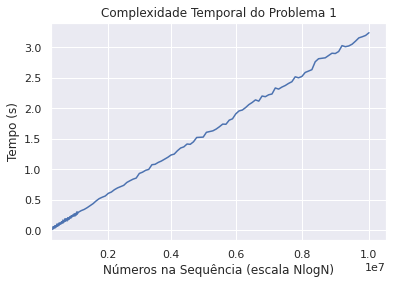
\includegraphics[width=0.4\textwidth]{report_prob1.png}
    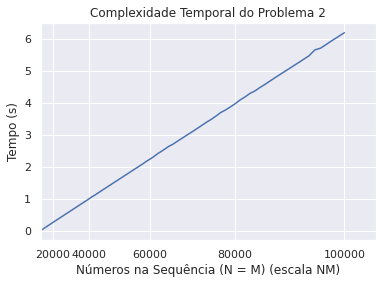
\includegraphics[width=0.4\textwidth]{report_prob2.png}
  \end{wrapfigure}

  Para o problema 1, foram utilizadas sequências de tamanho entre 10 e 100 000 000 elementos, 100 para cada ordem de grandeza.
  O gráfico apresentado à direita tem uma escala $N \log N$ no eixo dos $xx$.
  Os dados revelam uma reta linear, comprovando que a complexidade temporal do problema é efetivamente $O(N\log N)$, tal como concluido na análise teórica.

  Para o problema 2, por ser o pior caso e para simplificar a análise, tomou-se sempre $N = M$, ou seja, o mesmo número de elementos para ambas as sequências.
  Foram sempre utilizados números comuns, visto que esse é o pior caso no problema 2.
  Foram utilizadas sequências de tamanho entre 10 e 100 000 elementos, 100 para cada ordem de grandeza.
  O gráfico apresentado à direta tem uma escala $NM$ no eixo dos $xx$.
  Os dados revelam uma reta linear, comprovando que a complexidade temporal do problema é, num caso geral, $O(NM)$, tal como concluído na análise teórica.

  \section{Bibliografia}

  \printbibliography

\end{document}
